\scanpage{14}

% letterhead
of\\
Science\\
\figure{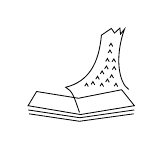
\begin{tikzpicture}[x=.45cm,y=.45cm,line width=.3pt]
\draw (0,0)--(.24,.4)--(1.42,.21)--(2.64,.45)--(3,0)--(1.48,-.25)--cycle;
\draw (0,-.12)--(1.46,-.34)--(3,-.12) (.03,-.23)--(1.45,-.44)--(2.98,-.23);
\draw (1.45,-.19)..controls (1.3,.25) and (1.25,.42)..(1.06,.52)
 ..controls (1.72,.68) and (2,1.21)..(2.07,1.99)
 --(2.35,2.18)--(2.44,2.05)--(2.59,2.19)--(2.61,2.02)
 --(2.72,2.16)..controls (2.43,1.35) and (2.57,.63)..(2.84,.46);
\foreach \x/\y in {1.6/.55,1.78/.6,1.91/.75,2.04/.9,2.16/1.04,2.19/1.25,2.26/1.49,2.29/1.68,2.03/.55,2.19/.67,2.31/.79,2.38/1.02,2.37/1.24,2.43/.55}
{\draw (\x,\y)--++(.05,.08)--++(.05,-.09);}
\end{tikzpicture}}
% crop-candidate: scan 14
NAGOYA UNIV.

名古屋大学内 \quad \unsure{日本郵便}\\
20.12.77 \quad NAGOYA DAIGAKUNAI \quad 0,340\\
H1208 \quad JAPAN

Professeur Alexandre Grothendieck\\
34700 Villecun (Lod\=eve)\\
\uline{FRANCE}

VIA AIR MAIL\\
PAR AVION

PAR AVION\\
航空郵便

\handwritten{\unsure{340|3X0}}

\handwritten{$\{\lambda,\lambda^{-1}\}\quad|\lambda|\ne1$\quad donc $\lambda\ne\lambda^{-1}$ i.e. $\lambda^2\ne1$ i.e. $\lambda\ne\pm1$ i.e. $\alpha\ne\pm2$}

\handwritten{$\lambda+\lambda^{-1}=\alpha$\qquad\deleted{\unsure{pte|qqc|tel que}} $\alpha\notin[-2,+2]$}
\[
\handwritten{\begin{aligned}
\alpha^2-4\qquad &\unsure{\nLeftrightarrow|\not\Leftarrow}\lambda\bar\lambda=1\\
&\bar\lambda=\lambda^{-1}\\
&\lambda+\lambda^{-1}\ \text{\uline{réel}}
\end{aligned}}
\]
% archive sheet number: 13
